Lors de la section sur l'implicit tiling \autoref{sec:implicit-tiling}, j'ai mentionné que l'implicit tiling créait les \texttt{bounding volumes} et les \texttt{geometric errors} de manière automatique. Ce n'est pas vraiment le cas. Par défaut, ils ne sont pas définis par l'implicit tiling, mais il est possible de rajouter l'extension \href{https://github.com/CesiumGS/3d-tiles/tree/main/extensions/3DTILES_bounding_volume_S2}{3DTILES\_bounding\_volume\_S2}\footnote{https://github.com/CesiumGS/3d-tiles/tree/main/extensions/3DTILES\_bounding\_volume\_S2} qui permet de compléter les tuiles générées par l'implicit tiling avec des \texttt{bounding volumes} et des \texttt{geometric errors} calculés automatiquement.

Sans trop rentrer dans les détails, l'extension utilise une \href{https://en.wikipedia.org/wiki/Hilbert_curve}{courbe de Hilbert}\footnote{https://en.wikipedia.org/wiki/Hilbert\_curve} sur une partition en plusieurs niveaux de tuiles faite par la librairie \href{http://s2geometry.io/}{S2 Geometry}\footnote{http://s2geometry.io/}. Ce sujet rentre dans la thématique des \href{https://en.wikipedia.org/wiki/Binary_space_partitioning}{Binary Space Partitioning}\footnote{https://en.wikipedia.org/wiki/Binary\_space\_partitioning}. Tout comme la partition du monde en 2 dimensions et son indexation avec un index de Motron qui sera vu dans la section \ref{sec:morton}, le partitionnement du monde peut aussi se faire avec la librairie S2 Geometry et son indexation avec une courbe de Hilbert. Ces deux méthodes sont donc des \textit{Binary Space Partitioning}. Ici, ces méthodes permettent de diviser une surface et permettent de donner rapidement et efficacement les informations spatiales des tuiles.

Pour utiliser cette extension, il suffit de rajouter les champs \texttt{extensionsUsed} et \texttt{extensionsRequired} dans le fichier JSON du Tileset. Puis, il faut rajouter une tuile dans le champ \texttt{children} du fichier JSON du Tileset. Cette tuile doit contenir un champ \texttt{boundingVolume} avec un champ \texttt{extensions} contenant les informations nécessaires pour l'extension.

Remarquez le champ \texttt{token} dans l'exemple ci-dessous. Il s'agit d'un identifiant unique correspondant à la \textit{root cell} (la cellule de plus haut niveau) de la courbe de Hilbert. Selon l'extension, le globe terrestre à été divisé en 6 \textit{root cells} comme si l'on avait projeté les 6 faces d'un cube sur la terre. Par exemple, l'Antarctique se trouve dans la cellule "5".

\newpage

Voici un exemple de fichier JSON utilisant l'extension 3DTILES\_bounding\_volume\_S2 :

\begin{verbatim}
{
    "asset" : {
        "version" : "1.1"
    },
    "geometricError": 1200000,
    "extensionsUsed": [
        "3DTILES_bounding_volume_S2"
    ],
    "extensionsRequired": [
        "3DTILES_bounding_volume_S2"
    ],
    "root" : {
        "boundingVolume": {
        "region": [-3.14159, -1.57079, 3.14159, 1.57079,
            0, 60
        ]
        },
        "refine": "REPLACE",
        "geometricError": 1200000,
        "children": [
        {
            "boundingVolume": {
            "extensions": {
                "3DTILES_bounding_volume_S2": {
                "token": "1",
                "minimumHeight": 0,
                "maximumHeight": 20
                }
            }
            },
            "refine": "REPLACE",
            "geometricError": 120000
        },
        ],
        "content": {
            "uri" : "/content/content_glb_{level}__{x}_{y}.glb"
        },
        "implicitTiling" : {
            "subdivisionScheme" : "QUADTREE",
            "subtreeLevels" : 4,
            "availableLevels" : 19,
            "subtrees" : {
                "uri" : "/subtrees/{level}.{x}.{y}.subtree"
            }
        }
    }
}
\end{verbatim}

\begin{figure}[H]
    \centering
    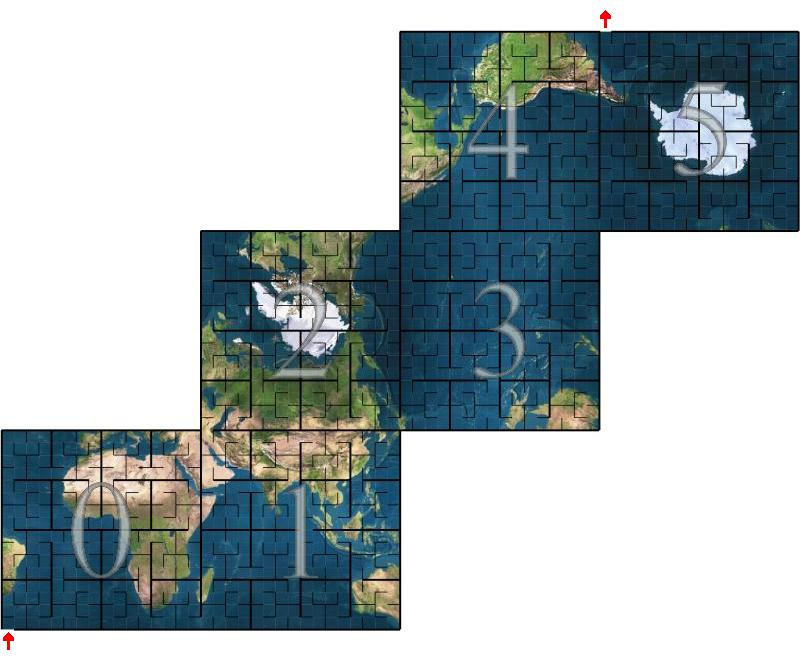
\includegraphics[width=1\textwidth]{assets/figures/s2cell_global.jpg}
    \caption{Tokens des 6 \textit{root cells} \cite{3DTILES_bounding_volume_S2-website}}
    \label{fig:s2-ext}
\end{figure}

Notez aussi que dans l'exemple JSON ci-dessus, qu'une seule \textit{root cell} est définie. Dans mon cas, comme j'aimerai pouvoir utiliser l'entièreté de la terre, j'ai défini les 6 \textit{root cells} en tant que 6 \texttt{children} différents avec chacun leur propre \texttt{token}.

Cette manière de partager l'espace de la terre ne correspond cependant pas à la méthode qu'utilise l'implicit tiling. Les calculs nécessairs pour convertir les indexes de l'implicit tiling vers ceux des courbes de Hilbert ne sont néanmoins pas à effectuer par nos soins, l'extension ce charge de cela.